% !Mode:: "TeX:UTF-8"
\chapter{Применение предлагаемых методов, сравнение с аналогами}

В этой главе показывается, что предлагаемых в диссертации средств моделирования микропроцессоров достаточно для генерации тестовых программ, нацеленных на подсистемы управления памяти, таких трех часто используемых архитектур как MIPS~\cite{mips64II}, PowerPC~\cite{PowerPC} и IA-32~\cite{IA32}. При рассмотрении архитектур важными будут следующие вопросы:
\begin{enumerate}
    \item описываются ли варианты исполнения инструкций в виде ограничений на битовые строки в документации (тогда трудоемкость моделирования вариантов исполнения инструкций была бы ниже);
    \item возможно ли моделирование устройств подсистемы управления памяти; существуют ли устройства, не моделируемые в виде таблиц;
    \item хватает ли предлагаемых в диссертации средств для описания трансляции адресов.
\end{enumerate}

В разделе~\ref{sec:templates_estimation} описаны эксперименты по оценке длины шаблонов, для
которых удается эффективно строить тесты предлагаемыми в диссертации
методами. Заканчивается глава
сравнением особенностей предлагаемого метода генерации тестовых программ по
тестовым шаблонам с методом, предлагаемым инструментом
Genesys-Pro~\cite{GenesysPro}, а также сравнение с некоторыми работами в Intel~\cite{MicroFORMAL}.

%% отвечаем на следующие вопросы:
% 1. описываются ли инструкции в виде ограничений на битовые строки в документации
% 2. описывается ли модель состояния MMU в виде лишь таблиц? нет ли там
% чего-нибудь, не сводящегося к таблице?
% -> структура TLB
% 3. хватает ли средств для описания трансляции адреса ?
% -> поток данных, описывающих трансляцию
% режимы работы (real mode, protected mode)

% таблица - то, что представляется множеством строк,
% строка представляется набором полей ключа и полей данных

%% схема описания компонента MMU:
% 1. поля строк
% 2. количество строк
% 3. битовая длина номера региона (тип таблицы - полностью-ассоциативная, ....)
% 4. стратегия вытеснения
% 5. предикат keyMatch
% 6. особенности компонента (чего-то более одного, чего-то быть не может, ...) -
% например, одна строка хранит несколько подряд данных

% в MIPS R12000 появилась кэш-память адресов переходов (32 строки), но она не
% относится к MMU данных

\section{Генерация тестов для архитектуры MIPS}\label{sec:mips_application}

%\begin{utv}
%Для архитектуры MIPS возможно применение применение методов, описанных в
% диссертации, для генерации тестовых программ по тестовым шаблонам; причем
% методов достаточно
% для полного описания поведения MMU микропроцессоров архитектуры MIPS.
%\end{utv}

Документация по архитектуре MIPS представлена в MIPS64™ Architecture For Programmers (в трех томах)~\cite{mips64II, mips64III}. Второй том (The MIPS64™ Instruction Set) содержит описания инструкций. Они  действительно описываются в виде набора операций над битовыми строками на специальном псевдокоде.% (см.рис.~\ref{fig:mips64_page}).

%\begin{figure}
%\framebox[0.93\textwidth][l]{\parbox{0.9\textwidth}{
%
%\textbf{Load Doubleword    LD}\\
%
%\textbf{Format:} LD rt, offset(base)\\
%
%\textbf{Purpose:} To load a doubleword from memory\\
%
%\textbf{Description:} rt <- memory[base+offset]
%
%The contents of the 64-bit doubleword at the memory location specified by the aligned effective address are fetched and placed in GPR rt. The 16-bit signed offset is added to the contents of GPR base to form the effective address.\\
%
%\textbf{Restrictions:}\\
%The effective address must be naturally-aligned. If any of the 3 least-significant bits of the address is non-zero, an Address Error exception occurs.\\
%
%\textbf{Operation:}
%
%\texttt{vAddr <- sign\_extend(offset) + GPR[base]}
%
%\texttt{if vAddr$_{2..0} \neq 0^3$ then}
%
%\hspace{2cm}\texttt{SignalException(AddressError)}
%
%\texttt{endif}
%
%\texttt{(pAddr, CCA) <- AddressTranslation (vAddr, DATA, LOAD)}
%
%\texttt{memdoubleword <- LoadMemory (CCA, DOUBLEWORD, pAddr, vAddr, DATA)}
%
%\texttt{GPR[rt] <- memdoubleword}\\
%
%\textbf{Exceptions:}\\
%TLB Refill, TLB Invalid, Bus Error, Address Error, Reserved Instruction, Watch
%
%}
%}
%\caption{Пример страницы документации по системе команд архитектуры MIPS64}\label{fig:mips64_page}
%\end{figure}

Третий том (The MIPS64™ Privileged Resource Architecture) содержит описание подсистемы управления памяти в
микропроцессорах MIPS. Для работы с данными она содержит следующие устройства (количественные
характеристики приведены для микропроцессора MIPS R10000~\cite{R10000}):
\begin{itemize}
  \item \emph{кэш-память данных первого уровня (D-Cache-1)}:
        \begin{itemize}
            \item размер: 32 кБ;
            \item поля строк: тэг физического адреса (ключ), данные (данные);
            \item битовая длина номера региона: 6 (наборно-ассоциативная\\ кэш-память);
            \item количество строк в регионе: 2;
            \item стратегия вытеснения \LRU;
        \end{itemize}
  \item \emph{кэш-память второго уровня (Cache-2)}:
        \begin{itemize}
            \item размер: от 512 кБ до 16 МБ;
            \item поля строк: тэг физического адреса для кэш-памяти второго
уровня (ключ), данные (данные) (16 или 32 слова);
            \item количество строк в регионе: 2;
            \item стратегия вытеснения \LRU;
        \end{itemize}
         Cache-2 является внешней;
  \item \emph{TLB (Joint-TLB)}:
        \begin{itemize}
            \item поля строк: r, vpn/2, g, asid (ключи), pfn0, cca0, v0, c0, d0,
pfn1, cca1, v1, c1, d1 (данные);
            \item битовая длина номера региона: 0 (полностью-ассоциативный TLB);
            \item количество строк в регионе: 64;
            \item вытеснение программное (т.е. стратегия вытеснения none);
            \item размер виртуального адреса: 44 бита;
            \item размер физического адреса: 40 бит;
        \end{itemize}
        одна строка TLB хранит информацию про две соседние страницы виртуальной
        памяти;
  \item \emph{буфер TLB (D-TLB)}:
        \begin{itemize}
            \item поля строк те же, что и для Joint-TLB;
            \item битовая длина номера региона: 0 (полностью-ассоциативный);
            \item количество строк в регионе: 8;
            \item стратегия вытеснения \LRU;
        \end{itemize}
\end{itemize}

Другие устройства для обращения в память не используются.

Осталось показать, что трансляция адреса также может быть представлена в виде
отношений на битовых строках и обращений в таблицы. Обычное выполнение
обращения к памяти в MIPS следующее:
\begin{enumerate}
    \item на основе аргументов инструкции формируется \emph{виртуальный адрес} (VA);
    \item заменой в виртуальном адресе номера страницы виртуальной памяти на номер фрейма физической памяти формируется \emph{физический адрес} (PA);
    \item по физическому адресу, если нужно, осуществляется обращение в кэш-память или обращение в оперативную память.
\end{enumerate}

\begin{figure}[h] \center
  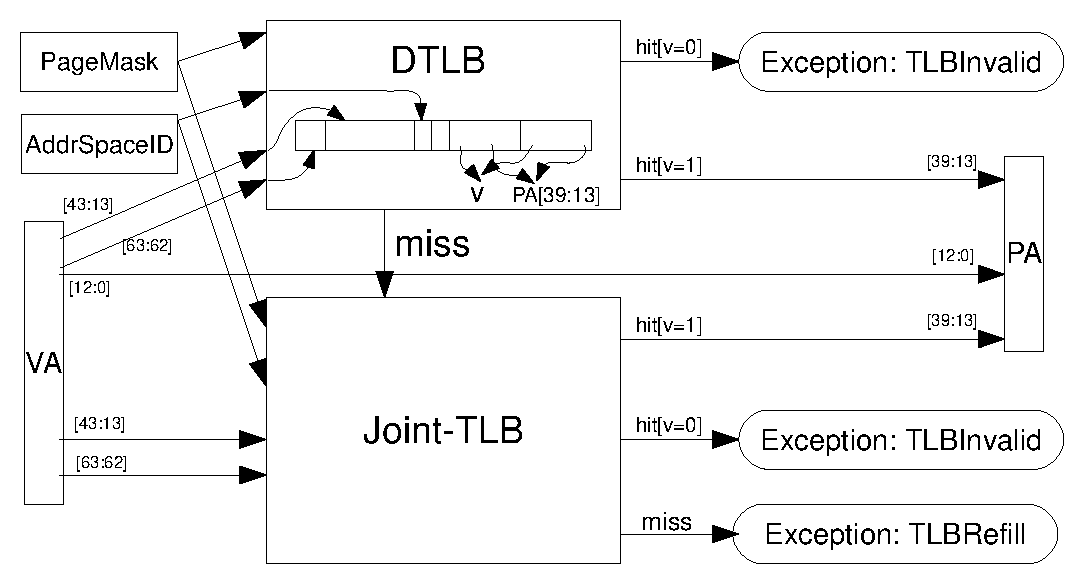
\includegraphics[width=0.8\textwidth]{4.analysis/mips_addrtrans}\\
  \caption{Трансляция адреса в MIPS}\label{fig:mips_address_translation}
\end{figure}


В зависимости от значения виртуального адреса и состояния управляющих регистров
возможны следующие варианты трансляции адреса:
\begin{itemize}
  \item для виртуального адреса трансляция проходит через TLB
(см.рис.~\ref{fig:mips_address_translation});
  \item для виртуального адреса трансляция проходит без таблиц (физический адрес
--- битовая строка --- является результатом битовых операций над виртуальным
адресом --- битовой строкой).
\end{itemize}

Пример модели инструкции LD с рисунка~\ref{fig:mips64_page} приведен в приложении~\ref{sec:xml}.

\section{Генерация тестов для архитектуры PowerPC}\label{sec:ppc_application}

Архитектура PowerPC разработана компанией IBM. Документация по архитектуре
PowerPC представлена в PowerPC Architecture Book (в трех томах)~\cite{PowerPC}. Первый том (PowerPC User Instruction Set Architecture) содержит описания инструкций. Они действительно описываются в виде набора операций над битовыми строками на специальном псевдокоде (см.рис.~\ref{fig:ppc_page}.

\begin{figure}
\framebox[0.93\textwidth][l]{\parbox{0.9\textwidth}{
\textbf{Store Halfword Indexed X-form}

sthx RS,RA,RB\\


\texttt{if RA = 0 then b <- 0}

\texttt{else \hspace{2cm}  b <- (RA)}

\texttt{EA <- b + (RB)}

\texttt{MEM(EA, 2) <- (RS)$_{48:63}$}\\

Let the effective address \texttt{(EA)} be the sum \texttt{(RA|0)+(RB)}. \texttt{(RS)$_{48:63}$} are stored into the halfword in storage addressed by \texttt{EA}.\\

\textbf{Special Registers Altered:}\\
None
}}
\caption{Пример страницы документации системы команд PowerPC}\label{fig:ppc_page}
\end{figure}

Третий том (PowerPC Operating Environment Architecture) содержит описание подсистемы управления памяти в микропроцессорах PowerPC. Для работы с данными она содержит следующие устройства (количественные характеристики приведены для микропроцессора PowerPC 970FX
~\cite{PowerPC970FXUserManual}):
\begin{itemize}
  \item \emph{кэш-память данных первого уровня (D-Cache-1)}:
        \begin{itemize}
            \item размер: 32 кБ;
            \item поля строк: тэг физического адреса (ключ), данные (данные);
            \item битовая длина номера региона: 7 (наборно-ассоциативная\\кэш-память);
            \item количество строк в регионе: 2;
            \item стратегия вытеснения \LRU;
        \end{itemize}
  \item \emph{кэш-память второго уровня (Cache-2)}:
        \begin{itemize}
            \item размер: 512 кБ;
            \item поля строк: тэг физического адреса (ключ), данные (данные);
            \item битовая длина номера региона: 11 (наборно-ассоциативная кэш~--~память);
            \item количество строк в регионе: 8;
            \item стратегия вытеснения \LRU;
        \end{itemize}
  \item \emph{D-TLB} (кэш таблицы страниц):
        \begin{itemize}
            \item поля строк: номер страницы виртуальной памяти (ключ), номер\\фрейма физической памяти (данные);
            \item битовая длина номера региона: 8 (наборно-ассоциативный);
            \item количество строк в регионе: 4;
            \item стратегия вытеснения \LRU;
        \end{itemize}
  \item \emph{сегментные регистры (SLB, Segment Lookaside Buffer)}:
        \begin{itemize}
            \item поля строк: effective segment id (ключ), virtual segment id
(данные), биты K$_s$/K$_p$, V, N, L, C (данные);
            \item битовая длина номера региона: 0 (полностью ассоциативный);
            \item количество строк в регионе: 64;
            \item вытеснение программное;
        \end{itemize}
        используются для получения виртуального адреса по эффективному;
%  \item \emph{буфер непосредственной трансляции адресов (D-ERAT)}:
% НЕТ ЭТОГО БУФЕРА В АРХИТЕКТУРЕ!!! его добавили в самом микропроцессоре
% PPC970FX
%        \begin{itemize}
%            \item поля строк: номер <<эффективной страницы>> (ключ), номер
% фрейма физической памяти (данные), биты (данные);
%            \item битовая длина номера региона: 6 (наборно-ассоциативная
% таблица);
%            \item количество строк в регионе: 2;
%            \item стратегия вытеснения \FIFO;
%        \end{itemize}
\end{itemize}

Кроме того, в оперативной памяти организуется \emph{таблица страниц виртуальной памяти (PageTable)}. Хотя формально она не является устройством подсистемы управления памяти, но используется при трансляции адресов, то она тоже может быть оформлена в виде такой таблицы:
    \begin{itemize}
        \item поля строк: номер страницы виртуальной памяти (ключ), номер фрейма
физической памяти (данные);
        \item битовая длина номера региона: 65;
        \item количество строк в регионе: 1;
        \item вытеснение программное;
        \item размер эффективного адреса: 64 бита;
        \item размер виртуального адреса: 65 бит;
        \item размер физического адреса: 42 бита;
    \end{itemize}

На самом деле таблица страниц виртуальной памяти организована в виде сложной
хэш-таблицы, но для тестирования этот момент не важен --- главное, что это
соответствие номеров страниц виртуальной памяти номерам фреймов физической
памяти, причем необязательно представлены все страницы виртуальной памяти.

Другие устройства для обращения в память не используются.

Осталось показать, что трансляция адреса также может быть представлена в виде
отношений на битовых строках и обращений в таблицы. Обычное выполнение
обращения к памяти в PowerPC следующее:
\begin{enumerate}
    \item на основе аргументов инструкции обращения к памяти формируется \emph{эффективный
адрес} (EA);
    \item заменой в эффективном адресе номера сегмента на его адрес из SLB получается
\emph{виртуальный адрес} (VA);
    \item заменой в виртуальном адресе номера виртуальной страницы в виртуальном адресе на номер
фрейма физической памяти получается \emph{физический адрес} (PA);
    \item по физическому адресу, если нужно, осуществляется обращение в
кэш-память иди, если данных по физическому адресу нет в кэш-памяти, обращение в
оперативную память.
\end{enumerate}

В зависимости от состояния управляющих регистров возможны следующие варианты
трансляции адреса:
\begin{itemize}
  \item real addressing mode (трансляция выключена); физический адрес
вычисляется по эффективному без обращения к каким-либо таблицам;
  \item режим с трансляцией адреса (см. рис.~\ref{fig:ppc_address_translation}).
\end{itemize}

\begin{figure}[h] \center
  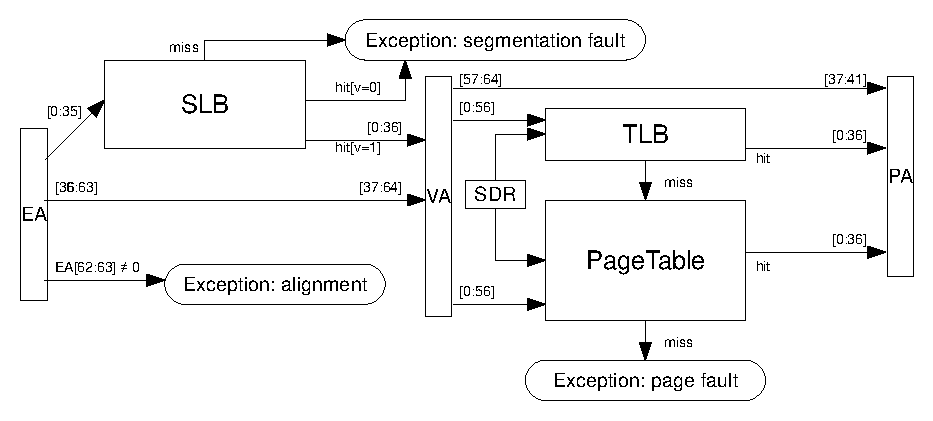
\includegraphics[width=\textwidth]{4.analysis/ppc_addrtrans}\\
  \caption{Трансляция адреса в PowerPC}\label{fig:ppc_address_translation}
\end{figure}


\section{Генерация тестов для архитектуры IA-32}\label{sec:ia32_application}

IA-32 --- это архитектура, разрабатываемая компанией Intel. Документация по
архитектуре IA-32 представлена книгой IA-32 Intel® Architecture
Software Developer’s Manual (в пяти томах)~\cite{IA32}. Второй и третий тома \\(Instruction Set Reference) содержат определения инструкций. Они действительно описываются в виде набора операций над битовыми строками на специальном псевдокоде. % (см. рисунок~\ref{fig:ia32_page}).

%\begin{figure}
%\framebox[0.93\textwidth][l]{\parbox{0.9\textwidth}{%
%
%\textbf{TEST—Logical Compare}\\
%
%\textbf{Description}\\
%Computes the bit-wise logical AND of first operand (source 1 operand) and the second operand
%(source 2 operand) and sets the SF, ZF, and PF status flags according to the result. The result is
%then discarded.\\
%
%\textbf{Operation}
%
%\texttt{TEMP <- SRC1 AND SRC2;}
%
%\texttt{SF <- MSB(TEMP);}
%
%\texttt{IF TEMP = 0}
%
%\hspace{1cm} \texttt{THEN ZF <- 1;}
%
%\hspace{1cm} \texttt{ELSE ZF <- 0;}
%
%\texttt{FI:}
%
%\texttt{PF <- BitwiseXNOR(TEMP[0:7]);}
%
%\texttt{CF <- 0;}
%
%\texttt{OF <- 0;}
%
%\texttt{(* AF is undefined *)}\\
%
%\textbf{Flags Affected}\\
%The OF and CF flags are set to 0. The SF, ZF, and PF flags are set according to the result (see
%the "Operation" section above). The state of the AF flag is undefined.
%}}
%\caption{Пример страницы документации системы команд архитектуры IA-32}\label{fig:ia32_page}
%\end{figure}

Четвертый и пятый тома (System Programming Guide) содержат описание подсистемы управления памяти в
микропроцессорах IA-32. Для работы с данными она содержит следующие устройства
(количественные характеристики приведены для микропроцессора Intel Pentium
Pro~\cite{PentiumPro}) :
\begin{itemize}
  \item \emph{кэш-память данных первого уровня (D-Cache-1)}:
        \begin{itemize}
            \item размер: 8 кБ;
            \item поля строк: тег адреса (ключ), данные (данные);
            \item битовая длина номера региона: 7 (наборно-ассоциативный);
            \item количество строк в регионе: 2;
            \item стратегия вытеснения \LRU;
        \end{itemize}

  \item \emph{кэш-память второго уровня (Cache-2)}:
        \begin{itemize}
            \item размер: в разных версиях 256 кБ, 521 кБ или 1 МБ;
            \item поля строк: тег адреса (ключ), данные (данные);
            \item битовая длина номера региона: от 11 до 13 в разных версиях
(наборно-ассоциативный);
            \item количество строк в регионе: 4;
            \item стратегия вытеснения \LRU;
        \end{itemize}

  \item \emph{TLB (D-TLB)}:
        \begin{itemize}
            \item поля строк: page number (ключ), page base address (данные),
флаги (данные);
            \item битовая длина номера региона: 4 (наборно-ассоциативный);
            \item количество строк в регионе: 4;
            \item стратегия вытеснения \LRU;
        \end{itemize}

  \item \emph{таблица страниц виртуальной памяти (PageTable)}:
    \begin{itemize}
        \item поля строк: page number (ключ), page base address (данные), флаги
(данные);
        \item битовая длина номера региона: 65;
        \item количество строк в регионе: 1;
        \item вытеснение программное;
        \item размер логического адреса: 48 бит;
        \item размер линейного адреса: 32 бит;
        \item размер физического адреса: 32 бита;
    \end{itemize}


  \item \emph{таблица дескрипторов сегментов (SDT)}:
        \begin{itemize}
            \item поля строк: segment selector (ключ), база (данные), флаги
(данные);
            \item битовая длина номера региона: 13;
            \item количество строк в регионе: 1;
            \item вытеснение программное;
        \end{itemize}
\end{itemize}

Другие устройства для обращения в память не используются.

\begin{figure}[h] \center
  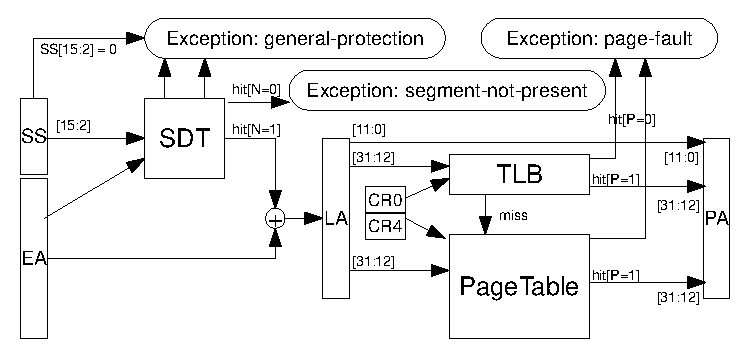
\includegraphics[width=0.8\textwidth]{4.analysis/ia32_addrtrans}\\
  \caption{Трансляция адреса в IA-32}\label{fig:ia32_address_translation}
\end{figure}

Осталось показать, что трансляция адресов также может быть представлена в виде
отношений на битовых строках и обращений в таблицы. Обычное выполнение
обращения к памяти в IA-32 следующее:
\begin{enumerate}
    \item на основе аргументов инструкции обращения к памяти формируется \emph{логический адрес} (SS:EA);
    \item заменой в логическом адресе номера сегмента на его адрес из SDT получается \emph{линейный адрес} (LA);
    \item либо линейный адрес трактуется как физический, либо заменой в линейном адресе номера виртуальной страницы на номер фрейма физической памяти получается физический адрес (PA);
    \item по физическому адресу, если нужно, осуществляется обращение в кэш-память или обращение в оперативную память.
\end{enumerate}

В зависимости от состояния управляющих регистров возможны следующие варианты трансляции адреса:
\begin{itemize}
  \item real-address mode (трансляция выключена) --- физический адрес равен линейному, линейный адрес вычисляется по логическому без обращения к каким-либо таблицам;
  \item protected mode --- режим с трансляцией адреса через таблицу страниц (см. рис.~\ref{fig:ia32_address_translation}).
\end{itemize}



\section{Экспериментальная реализация програм-\\много средства для генерации тестовых программ}

Был реализован прототип программного средства для генерации тестовых программ. Для проведения экспериментов к нему был добавлен генератор тестовых шаблонов. Компоненты прототипа программного средства для генерации тестовых программ следующие: %(см. рисунок~\ref{fig:activities}):
%\begin{figure}[h] \center
%  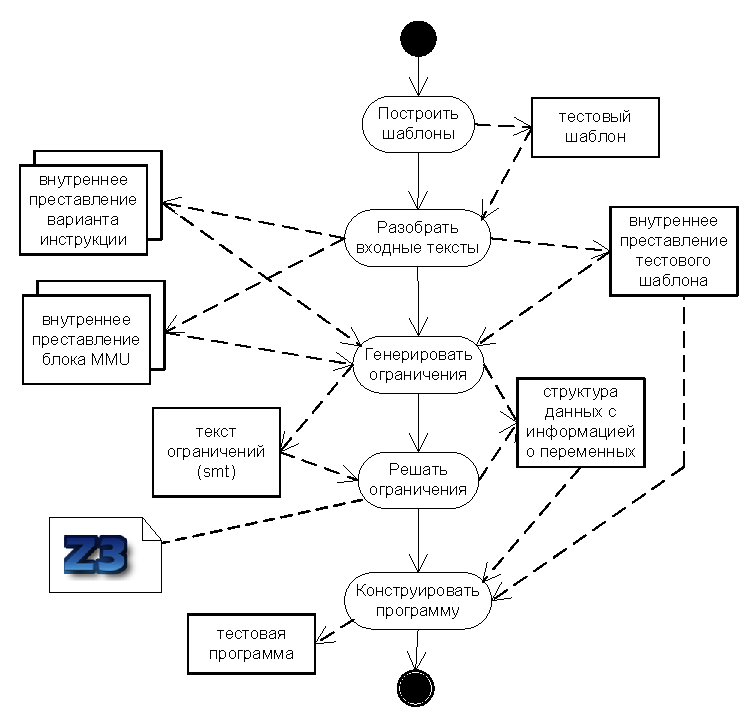
\includegraphics[width=0.7\textwidth]{3.impl/activities1}\\
%  \caption{Диаграмма деятельностей по генерации тестовых программ}\label{fig:activities}
%\end{figure}
\begin{enumerate}
  \item генератор тестовых шаблонов;
  \item синтаксический анализатор исходных текстовых данных; прототип генератора тестовых программ принимает на вход тексты в виде xml, создает внутреннее представление шаблона, моделей устройств, моделей вариантов инструкций для других компонентов;
  \item генератор (текстов) ограничений с использованием описанных в разделах~\ref{sec:constraints_generation_section} и \ref{sec:usefulness_functions} методов: прототип генератора тестовых программ генерирует тексты ограничений в формате SMT-LIB~\cite{SMT}; этот формат поддерживается большинством SMT-решателей ограничений, что делает возможным использовать разные внешние решатели ограничений и сравнивать их производительность применительно к генерируемым ограничениям; кроме того генератор строит структуры, хранящие семантическую информацию о переменных в ограничениях;
  \item обертка решателя ограничений: вызывает внешний решатель ограничений, считывает результат его работы, извлекает из этого результата значения переменных и сохраняет эти значения в созданной генератором текстов ограничений структуре;
  \item конструктор текстов тестовых программ на основе внутреннего представления шаблона и значений переменных.
\end{enumerate}

Часть компонентов зависит от тестируемого микропроцессора, а часть компонентов независима. К первым относятся конструктор текстов тестовых программ, поскольку он использует особенности, Специфичные для отдельных микропроцессоров или семейств микропроцессоров. Остальные компоненты не зависят от тестируемого микропроцессора и без изменений используются в генераторах тестов других микропроцессоров.

В прототипе синтаксический анализатор моделей, генератор текстов ограничений, обертка решателя ограничений были реализованы на Ruby (порядка 2000 строк). В качестве решателя ограничений был выбран инструмент Z3~\cite{Z3}, поскольку этот инструмент имеет лучшие параметры эффективности среди других инструментов.

В качестве архитектуры тестируемых микропроцессоров для экспериментов был выбран MIPS64, отчасти из-за наличия готовых компонент для проведения тестирования и моделей микропроцессоров. Конструктор тестовых программ для MIPS64 был реализован на Java (порядка 500 строк). Типичные размеры моделей варианта инструкции --- 100 строк (в представлении на xml). Типичный размер моделей устройства --- 20 строк (в представлении на xml). Эти модели подготавливаются вручную на основе документации по микропроцессору.

\section{Эксперименты по оценке допустимой сложности тестовых шаблонов}\label{sec:templates_estimation}

%эксперименты с длинами и временем генерации/процентом успешной
%генерации. Показать, что допустимая длина действительно увеличивается!

Хотя теоремы о корректности и полноте методов генерации ограничений гарантирует, что тестовая программа для тестового шаблона существует тогда и только тогда, когда совместна система ограничений. Однако не всегда совместность можно определить за ограниченное время (поскольку требуется строить тестовые программы для определенного количества тестовых ситуаций за вполне ограниченное, выделенное на это время в рамках проектов по тестированию моделей микропроцессоров). Из очевидных соображений чем <<сложнее>> тестовый шаблон, тем больше требуется времени на построение тестовой программы по нему (и определения того, что тестовая программа существует). Под сложностью понимается степень зависимости параметров тестового шаблона. Чем больше зависимостей, тем сложнее тестовый шаблон. Чем меньше зависимостей, тем продуктивнее будет воспользоваться более простыми целенаправленными методами получения тестовых программ, нежели предлагаемые в диссертации. Поэтому важно иметь оценку допустимой <<сложности>> тестовых шаблонов, исходя из реальных решателей и реальных тестируемых микропроцессоров.

Для получения таких оценок был проведен ряд экспериментов. В экспериментах тестовые шаблоны состояли из инструкций загрузки и сохранения
данных в памяти. В каждой инструкции должна была выполняться трансляция адреса
через TLB (с использованием D-TLB) и затем обращение в основную память через
кэш-память первого уровня. Вариант исполнения инструкций загрузки и сохранения задавался парой параметров: успешность обращения в TLB и успешность обращения в кэш-память. Модель вариантов инструкции загрузки LD приведена в приложении~\ref{sec:xml}. Рассматривались все длины тестовых шаблонов от 2 до
16. Для каждой длины проводились эксперименты для разных моделей микропроцессоров: они отличались ассоциативностью кэш-памяти. Использовались значения ассоциативности --- 2, 4, 8 и 16. При фиксированной длине шаблона и ассоциативности кэш-памяти случайным образом генерировался тестовый шаблон (т.е. случайным образом выбирались зависимости аргументов инструкций и варианты исполнения для инструкций). Количество тестовых шаблонов имело порядок тысяч шаблонов. Далее в этом разделе проводится статистический анализ для обоснования выбранного количества тестовых шаблонов для экспериментов.

Эксперименты проходили на компьютере AMD Athlon64 3200+ 2ГГц с 1ГБ оперативной памяти.

Рисунки~\ref{fig:success_experiment} и~\ref{fig:time_experiment} представляют
результаты экспериментов. На рисунке~\ref{fig:success_experiment} отражена доля
шаблонов, для которых была построена тестовая программа за время, меньшее чем 60 секунд или был получен сигнал о том, что тестовой программы не существует (если время превышало 60 секунд, построение тестовой программы обрывалось). На рисунке~\ref{fig:time_experiment} отражено среднее арифметическое времени генерации тестовой программы. Более точно, среднее время определения того, что шаблон <<является несовместным>> (для него не может быть теста вовсе) или
совместным с построением теста. Большую часть времени занимало разрешение ограничений.


\begin{figure}[p] \center
\parbox[t]{0.9\textwidth}{
  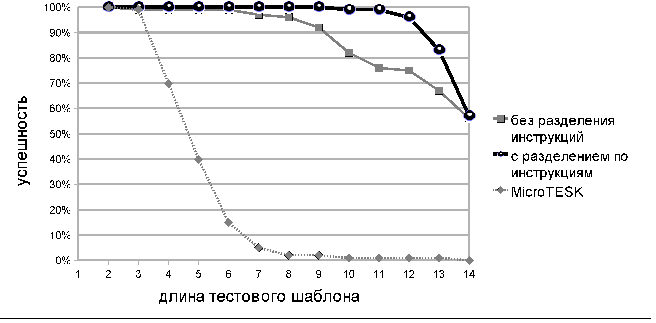
\includegraphics[width=0.9\textwidth]{4.analysis/success_exprmnt}%
\caption{Доля тестовых шаблонов, для которых удалось построить тестовую программу за 60с или определить их несовместность}\label{fig:success_experiment}
}

\vspace{1.5cm}

\parbox[t]{0.9\textwidth}{
  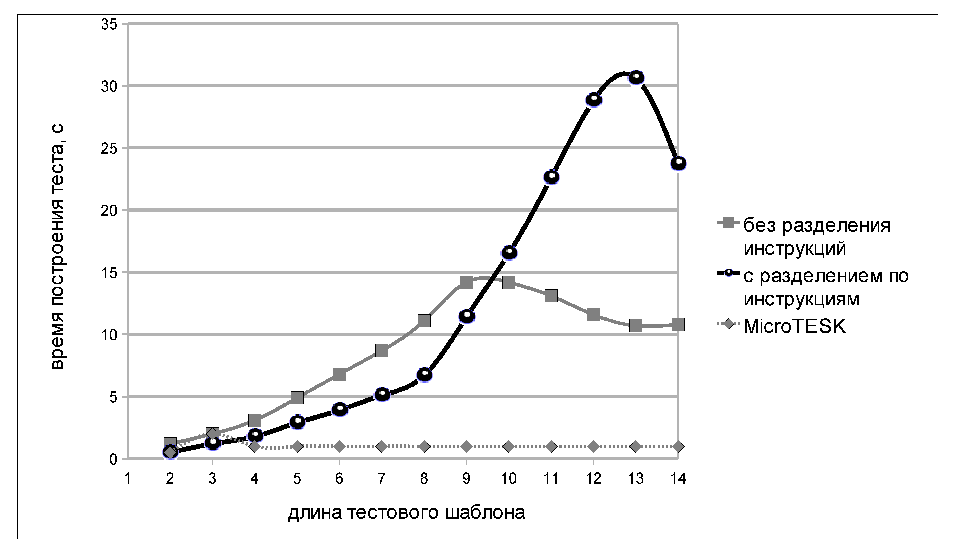
\includegraphics[width=0.9\textwidth]{4.analysis/time_exprmnt}
  \caption{Среднее время построения тестовой программы / определения несовместности тестового шаблноа}\label{fig:time_experiment}
}
\end{figure}

В первой серии экспериментов (их результаты отражены на рисунках линиями с
квадратиками) генерация ограничений делалась для всего тестового шаблона.
Оказалось, что до некоторой длины шаблона (значит, и теста) (8-9) метод работает
успешно практически для всех тестовых шаблонов (97\%-100\%). При дальнейшем
увеличении длины шаблона начинает уменьшаться доля шаблонов, для которых удается
построить тест (по 5-10\% при увеличении длины теста). Тем самым при длине теста
порядка 14-15 уже для половины шаблонов решатель ограничений не успевает за 60
секунд обработать тестовый шаблон (и построить тест). В результате анализа использованных в
экспериментах тестовых шаблонов был сделан вывод, что для большинства из них
(60-70\%) тестов не может быть вовсе, так как в этих шаблонах имеются пары расположенных подряд обращений
по одинаковым адресам, при этом первое обращение --- успешное или неуспешное, а второе --- успешное. Для таких шаблонов не существует тестовых программ (поскольку в результате промаха данные помещаются в таблицу и при повторном обращении к ним должно происходить только попадание, а не промах).

Поскольку эта ситуация стала по сути следствием случайного выбора тестовых
шаблонов, то в следующей серии экспериментов перед запуском генерации
ограничений была вставлена процедура, отсеивающая априори несовместные тестовые
шаблоны (т.е. такие, для которых не может существовать тестов вовсе). Кроме того
обращения в кэш-память были поделены на группы на основе одинаковых имен
аргументов и для этих групп генерировались ограничения (грубо говоря, к шаблону
добавлялось требование обращения по разным именам аргументов в разные регионы,
если это не противоречило шаблону). Результаты этой второй серии экспериментов
отражены на рисунках~\ref{fig:success_experiment} и \ref{fig:time_experiment}
линией с кружками. Из них следует, что примененные изменения позволили
дополнительно увеличить на несколько единиц допустимый размер тестового шаблона.

Для каждой пары (длина шаблона, ассоциативность) было сгенерировано 1000
тестовых шаблонов. Насколько можно доверять полученным в экспериментах
результатам на таком количестве тестовых шаблонов? Для ответа на этот вопрос воспользуемся аппаратом теории
вероятностей. Пусть $N$ --- количество испытаний. Одно испытание заключается в
следующем: сначала случайным образом строится тестовый шаблон, затем генерируются
для него ограничения и, наконец, они разрешаются. Испытание заканчивается успешно, если за отведенное время (60с) решатель ограничений <<построил тест>>, и неуспешно, если не успел <<построить>>.
Обозначим  $\xi_i$, $i = 1, 2, \dots, N$, случайные величины, соответствующие
успешности испытаний. Их областью значений будет множество $\{0, 1\}$. Эти
случайные величины независимы и одинаково распределены (обозначим $p =
\mathsf{P}\{\xi_i = 1\}$). Поэтому применим \emph{закон больших чисел}, согласно
которому $\frac{\sum_{i=1}^N \xi_i}{N} \sim p$ при <<больших>> $N$. Более точно, для любых
положительных $\varepsilon$ и $\delta$ найдется число $N^*$, что для всех $N > N^*$ будет
выполнено $\mathsf{P}\{|\frac{\sum_{i=1}^N \xi_i}{N} - p | \geq \varepsilon\} \leq \delta$. $\varepsilon$ --- это допустимое отклонение в оценке результата экспериментов (т.е. оценке $p$). $\delta$ показывает, насколько можно доверять полученному результату экспериментов. Поскольку $\sum \xi_i$ распределена по биномиальному закону ($\mathsf{P}\{\sum_{i=1}^N \xi_i = m\} = \binom{N}{m} p^m (1{-}p)^{N{-}m}$), то для вероятности отклонения более, чем на $\varepsilon$, справедлива следующая формула: $$\sum_{m = 0}^{(p-\varepsilon)N} \binom{N}{m} p^m (1{-}p)^{N{-}m} + \sum_{m = (p+\varepsilon)N}^N \binom{N}{m} p^m (1{-}p)^{N{-}m} \leq \delta$$ Эта формула позволяет оценить $\delta$ при разных $p$, зная $\varepsilon$ и $N$.

Итак, для каждого $n \in \{2,3\}$ ($n$ --- длина тестового шаблона) было сгенерировано по $B = 1000$ тестовых шаблонов. При этом получилось $p \in [0.9, 1.0]$. Если взять допустимое отклонение от истинного значения $\varepsilon = 0.02$ (2\%) (что вполне допустимо, т.к. отклонение в 2\% не сильно изменит результат эксперимента), то вероятность ошибиться в этом случае была бы не более $\delta = 0.03$, т.е. 3\%, что тоже вполне допустимо. Для $n \in \{4, 5, 6, 7\}$ было сгенерировано по $N = 2000$ тестовых шаблонов (для $w \in \{2,4\}$). Если взять $\varepsilon = 0.02$ (2\%), то для $p \in [0.9, 1.0] ~ \delta{=}0.003$, т.е. $0.3\%$, т.е. ошибка в этом случае еще меньше. И, наконец, для $n \in \{8, 9, ..., 14\}$ было сгенерировано по $N = 3000$ тестовых шаблонов, что при $\varepsilon = 0.02$ и $p \in [0.5, 1.0]$ дает $\delta = 0.02$, т.е. всего 2\%. Таким образом, вероятность ошибки в проведенных экспериментах невелика.

Проведенные эксперименты позволяют произвести сравнение с инструментом
MicroTESK~\cite{MicroTESK}. Этот инструмент был успешно применен для построения
тестов по всевозможным тестовым шаблонам из 2-3 инструкций~\cite{vorobyev}. При
увеличении длины тестового шаблона (и, соответственно, его <<сложности>>) удается
строить тесты для всё меньшего количества шаблонов. Что и отражено на
рисунках~\ref{fig:success_experiment} и \ref{fig:time_experiment} линиями с
ромбами. Напротив, как показывают эксперименты, предложенные методы позволяют
строить тесты по шаблонам из 8-11 инструкций обращения к памяти. Допустимая
длина шаблонов может быть еще больше, если кроме инструкций обращения к памяти в
шаблоне используются и другие инструкции (например, арифметические).

\section{Сравнение с Genesys-Pro}

В разделе~\ref{sec:templates_estimation} было произведено сравнение предлагаемых в диссертации методов генерации тестовых программ с методами, реализованными в инструменте
MicroTESK~\cite{MicroTESK}. В этом разделе будет произведено сравнение с другим
инструментом целенаправленной генерации тестовых программ --- Genesys-Pro~\cite{GenesysPro} --- по организации генератора, производительности, организации входных данных и др. Сравнить
по эффективности экспериментальным способом с Genesys-Pro не удается, поскольку этот инструмент не распространяется за пределы IBM. Сравнение по другим характеристикам проводилось на основе  публикаций~\cite{GenesysPro2004Innovations, GenesysSolver}.

Технологически подготовка к генерации тестов с использованием Genesys-Pro выглядит следующим образом:
\begin{enumerate}
    \item подготовить Architectural simulator --- эталонный симулятор микропроцессора;
    \item подготовить Architectural model --- описание системы команд тестируемого микропроцессора с указанием для каждой инструкции набора атрибутов и ограничений значений атрибутов (по сути, описание в виде ограничений предусловия инструкции и вычисляемой ею функции); пример описания инструкции загрузки из памяти LoadWord изображен на рисунке~\ref{fig:GenesysProArchitecturalModel}; для описания трансляции адреса предлагается метод\\DeepTrans~\cite{DeepTrans} --- пример изображен на рисунке~\ref{fig:DeepTransExample};
    \item подготовить Testing knowledge --- комплект ограничений на аргументы инструкций, задающих <<интересные для тестирования>> соотношения значений и аргументов;
    \item подготовить Test template --- тестовый шаблон; в нем задается последовательность инструкций тестовой программы и, возможно, ограничения из Testing Knowledge (см. пример тестового шаблона на рисунке~\ref{fig:genesysPro_template});
    \item подготовить или использовать имеющийся решатель ограничений;
%    \item запустить Genesys-Pro с подготовленными моделями.
\end{enumerate}
%% я понимаю, что такую последовательность шагов нельзя называть
%% технологической, ибо непоятно
%% 1) как выбирать Testing knowledge - что туда включать, а что нет; наверняка,
%% есть некое понимание того, что хочется протестировать; это понимание
%% должно быть формализовано (модель покрытия) и на его основе уже решать,
%% что включать в Testing knowledge, а что нет;
%% 2) не описано, как анализировать результаты Genesys-Pro: всё ли он сделал или
%% нет, надо ли дорабатывать то, что он генерирует? Надо ли как-то иначе
%% формулировать модели с шагов 1-3 для того, чтобы тесты были построены
%% целиком. И что значит "целиком"? Нет ведь модели покрытия!

\begin{figure}[h] \center
  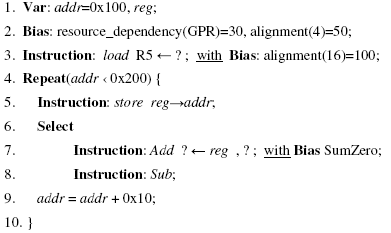
\includegraphics[width=0.6\textwidth]{4.analysis/genesys_tmpl}
  \caption{Пример тестового шаблона в нотации инструмента Genesys-Pro}\label{fig:genesysPro_template}
\end{figure}

\begin{figure}[h] \center
  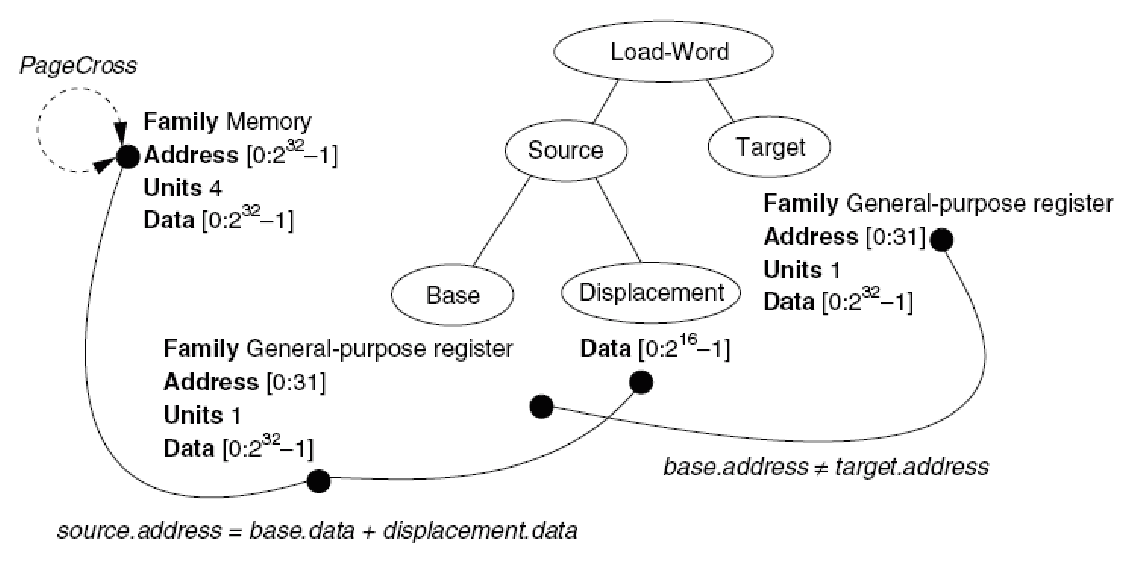
\includegraphics[width=0.8\textwidth]{4.analysis/arch-model}
  \caption{Architectural model для инструкции
LoadWord}\label{fig:GenesysProArchitecturalModel}
\end{figure}

\begin{figure}[h] \center
  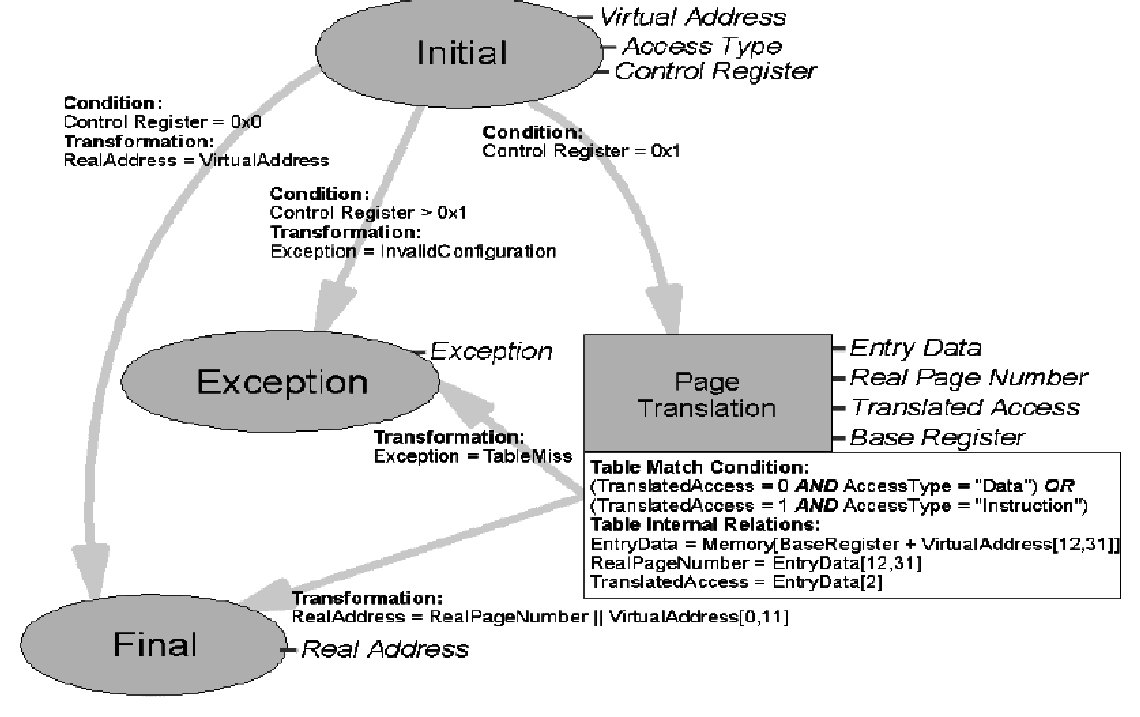
\includegraphics[width=0.8\textwidth]{4.analysis/deeptrans}
  \caption{Пример описания трансляции адреса по методу DeepTrans в инструменте Genesys-Pro}\label{fig:DeepTransExample}
\end{figure}

\begin{figure}[h] \center
  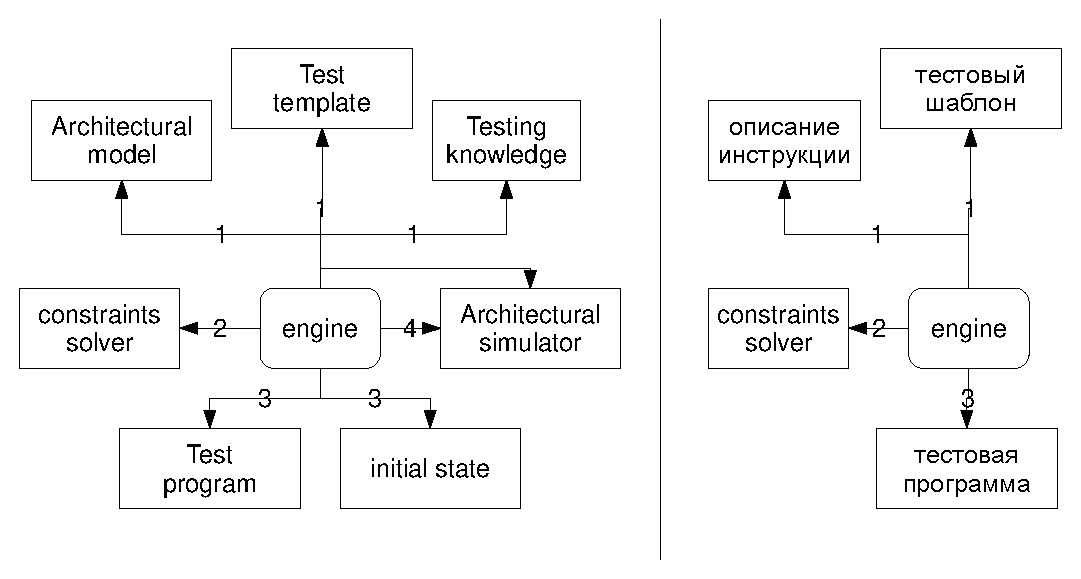
\includegraphics[width=\textwidth]{4.analysis/g-pro}
  \caption{Genesys-Pro (слева) и предлагаемый в диссертации генератор (справа)}\label{fig:GenesysProScheme}
\end{figure}

Genesys-Pro строит тестовую программу, чередую построение очередной инструкции и симуляцию этой инструкции, при этом каждый раз уточняя начальное состояние микропроцессора. Если построить очередную инструкцию невозможно (не удается подобрать параметры), происходит возврат на шаг назад и перегенерируется предыдущая инструкция. Аргументы каждой инструкции должны в текущем состоянии модели микропроцессора удовлетворять ограничениям из Architectural model и Testing knowledge. Для получения таких аргументов составляются системы ограничений и разрешаются встроенным решателем ограничений.

% т.е. получается, симулятор должен быть каким-то особенным, чтобы уметь
% работать из неполного состояния? (с lazy-значениями 'X') поскольку не
% всё начальное состояние построено перед
% первой инструкций и достраивается в процессе построения теста

Тем самым у предлагаемого в диссертации подхода, моделей и методов имеются следующие сходства с Genesys-Pro:
\begin{itemize}
    \item присутствуют способы указания ограничений на значения аргументов отдельных инструкций в тестовом шаблоне (здесь эти ограничения описываются в  виде вариантов исполнения инструкций, а в Genesys-Pro эти ограничения описываются в тестовом шаблоне и Testing knowledge);
    \item тестовый шаблон и микропроцессор описываются декларативным образом;
    \item оба подхода относятся к <<моделеориентированным>> --- в таких подходах есть генератора, на вход который принимает модель микропроцессора; альтернативой могла быть технология, в которой по модели вручную приходилось бы реализовывать на каком-нибудь языке программирования ряд специальных компонентов (в том числе учитывающие особенности модели микропроцессора и тестового шаблона), которые вместе дадут генератор тестовых программ;
    \item использование техники ограничений (constraints) для построения тестовых программ;
    \item сходные идеи есть и в методе описания трансляции адресов: в обоих случаях -- это декларативное описание, в обоих случаях описывается то, как формируются виртуальные/физические адреса; в обоих случаях описание трансляции основывается на представлении содержимого устройств подсистемы управления памяти в виде массивов данных, для которых задается ряд атрибутов (в том числе в Genesys-Pro есть аналог предиката keyMatch).
\end{itemize}

Имеются следующие отличия подходов:
\begin{itemize}
    \item разные принципы построения тестовых программ и ограничений; Genesys-Pro строит ее по одной инструкции и формулирует ограничения только для одной очередной инструкции; напротив, в предлагаемом методе ограничения строятся для всего тестового шаблона целиком;
    \item разные методы построения ограничений; при генерации системы ограничений Genesys-Pro существенно использует известную часть состояния микропроцессора (от Architectural simulator); напротив, в предлагаемом методе построения ограничений состояние микропроцессора неизвестно вообще; это приводит к ограничениям разной природы;
    \item Genesys-Pro предполагает для инструкции раздельное описание вычисляемой функции и ограничений на входные данные; в предлагаемом методе эти описания оформляются вместе;
    \item язык описания тестовых шаблонов в Genesys-Pro позволяет компактно описать длинные тестовые программы (из сотен тысяч инструкций), кроме того этот язык позволяет описывать классы тестовых шаблонов;
    \item разный способ описания функциональности инструкций; у Genesys-Pro --- это система ограничений на атрибуты инструкции и ее аргументы, а здесь --- это последовательность операторов;
    \item Genesys-Pro рассчитан на подготовку специальных решателей ограничений (из-за специфики его систем ограничений); напротив, в предлагаемом методе используются сторонние решатели ограничений и отдельно подготавливать их не нужно.
\end{itemize}

Преимущества и недостатки по сравнению с Genesys-Pro следующие:
\begin{itemize}
    \item Genesys-Pro поддерживает тестовые шаблоны, задающие цепочки инст{-}рукций из сотен и тысяч инструкций, т.е. он обладает преимуществом по длине генерируемых тестовых программ; однако такие тестовые шаблоны содержат существенно меньше зависимых параметров, нежели сотни и тысячи, поскольку шаблоны представляют собой итерацию конечных небольших последовательностей зависимых инструкций (см. рисунок~\ref{fig:genesysPro_template});
    \item преимуществом предлагаемого в диссертации подхода является меньшая трудоемкость подготовки генератора тестовых программ (как минимум, потому что не нужно разрабатывать решатель ограничений);
    \item возможность построения ограничений целиком для всего шаблона в предлагаемых методах дает преимущество перед построением по одной инструкции в Genesys-Pro по времени построения тестовой программы, например, для тестового шаблона с такой последовательностью инструкций: одна из инструкций вытесняет специальные данные (например, их тег адреса делится на 16) --- если Genesys-Pro не обеспечит таких данных, ему придется делать возвраты к предыдущим инструкциям (причем не на одну инструкцию, а несколько).
\end{itemize}

%Genesys-Pro чётко разделяет свойства аргументов
%инструкции и свойства результата инструкции, соотношение между ними
%задается не с помощью ограничений (т.е. не декларативным способом),
%а в виде алгоритма (т.е. императивным способом).
%
%Другой особенностью Genesys-Pro является то, что поддерживаемые им
%тестовые шаблоны зачастую не фиксируют последовательность инструкций
%(это позволяет строить более простые ограничения, потому как
%генерируемая последовательность инструкций может по ходу генерации
%подстраиваться под уже сгенерированные инструкции со
%сгенерированными значениями аргументов, под состояние
%микропроцессора, в которое привели сгенерированные инструкции).
%
%Выразительный язык Genesys-Pro для описания ограничений однако
%содержит такие нетривиальные конструкции, как явное использование
%элементов массивов данных, что требует для разрешения продвинутый
%решатель CSP, в том числе и заточенный под особенности генерации
%тестовых данных для тестовых шаблонов (как минимум такие ограничения
%могут включать битовые операции). Подобный решатель был разработан в
%IBM для инструмента Genesys-Pro~\cite{GenesysSolver}. Однако
%создание такого решателя -- отдельное сложное исследование, которое
%не входило в цели данного исследования. В данной работе было принято
%решение использовать доступные существующие решатели (не обязательно
%CSP) и сосредоточиться на упрощении генерируемых ограничений для
%некоторых частных случаев архитектур.
%
%%\begin{figure}[h]
%%\parbox{0.5\textwidth}{ \centering
%%  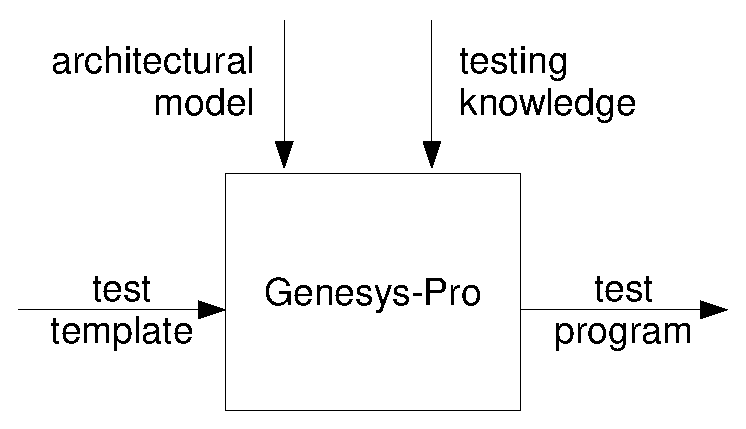
\includegraphics[width=0.45\textwidth]{3.impl/genesys-pro}
%%} \vline
%%\parbox{0.5\textwidth}{ \centering
%%  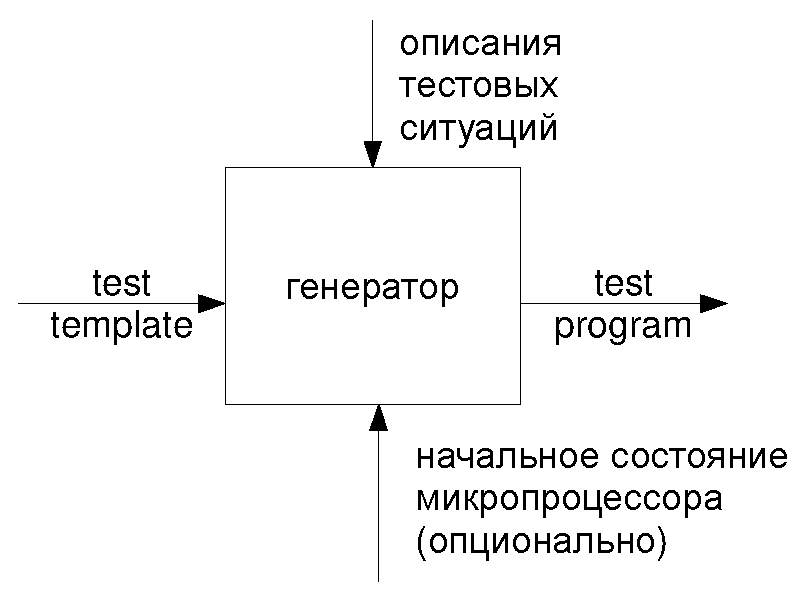
\includegraphics[width=0.45\textwidth]{3.impl/mygen}
%%}
%%\caption{Сравнение с Genesys-Pro}\label{comparison_genesyspro}
%%\end{figure}
%
%В отличие от Genesys-Pro в предлагаемом инструменте описание
%семантики инструкций задается в едином виде -- в виде описаний
%тестовых ситуаций~\cite{my_syrcose_2008, my_isp_2008}. Каждая
%тестовая ситуация описывает не только ограничение на свои аргументы,
%но и результат исполнения инструкции \emph{при данном ограничении на
%аргументы} инструкции декларативным образом. В функции, которую
%реализует инструкция, выделяются отдельные \emph{ветви
%функциональности}, ситуации различного поведения инструкций, каждая
%ветвь функциональности становится отдельной тестовой ситуацией.
%Например, инструкция целочисленного сложения ADD может быть
%исполнена либо точно, либо с возникновением переполнения. Поэтому у
%этой инструкции можно выделить 2 ветви функциональности (точное
%исполнение и исполнение с переполнением), каждая ветвь дает свою
%тестовую ситуацию.

\section{Сравнение с работами Intel}

В ряде публикаций~\cite{MicroFORMAL} описывается инструмент MicroFORMAL, разрабатываемый в Intel. Он используется для некоторых задач формальной верификации разрабатываемых микропроцессоров (в частности, для проверки обратной совместимости). В рамках этой работы требуется описывать поведение микропроцессоров, формализовывать функциональность инструкциЙ. Авторы статей разработали \emph{IRL-представление} микрокода (IRL --- Intermediate Representation Language). Спецификация на IRL описывает функциональность инструкции и побочный эффект (изменение <<внешних>> переменных). Ровно ту же цель преследуют и модели вариантов исполнения инструкций, предлагаемые в данной работе. Спецификация на IRL представляет собой последовательность операторов (эта же идея используется здесь).

IRL включает в себя управляющие операторы (\texttt{if}, \texttt{goto}), поскольку верификация с использованием спецификаций на IRL нацелена в первую очередь на верификацию потоков управления. В данной работе поток управления не предполагает подобных операторов.

IRL позволяет описывать инструкции обращения к памяти. Однако в IRL используется лишь <<плоская>> модель памяти (т.е. память рассматривается как одномерный массив ячеек) с возможностью обращения <<по индексу>>. Напротив, модели инструкций, предлагаемые в данной работе, позволяют описывать работу с памятью более детально, с указанием успешности обращений в различные устройства подсистемы управления памяти.
